\section*{Preliminary}\label{sec:preliminary}
\addcontentsline{toc}{section}{Preliminary}

\subsubsection*{Summary of the complete system}
% - http://www.math.sinica.edu.tw/www/tex/IPE_manual.pdf
In the navigation of the cargo ship several reference frames are used. Here we only consider two coordinate systems 'NED' and 'BODY'. NED is a coordinate system which lies on top of earths longitudinal and latitudinal axes with the z axis pointed downward into the center of the earth. BODY is places along the ship, with the x-axis from aft to fore, and y-axis from port to starboard side and z-axis from top to bottom. \cref{fig:boat_coordsys} illustrates the BODY and NED reference frames.
\begin{figure}[H]
    \centering
    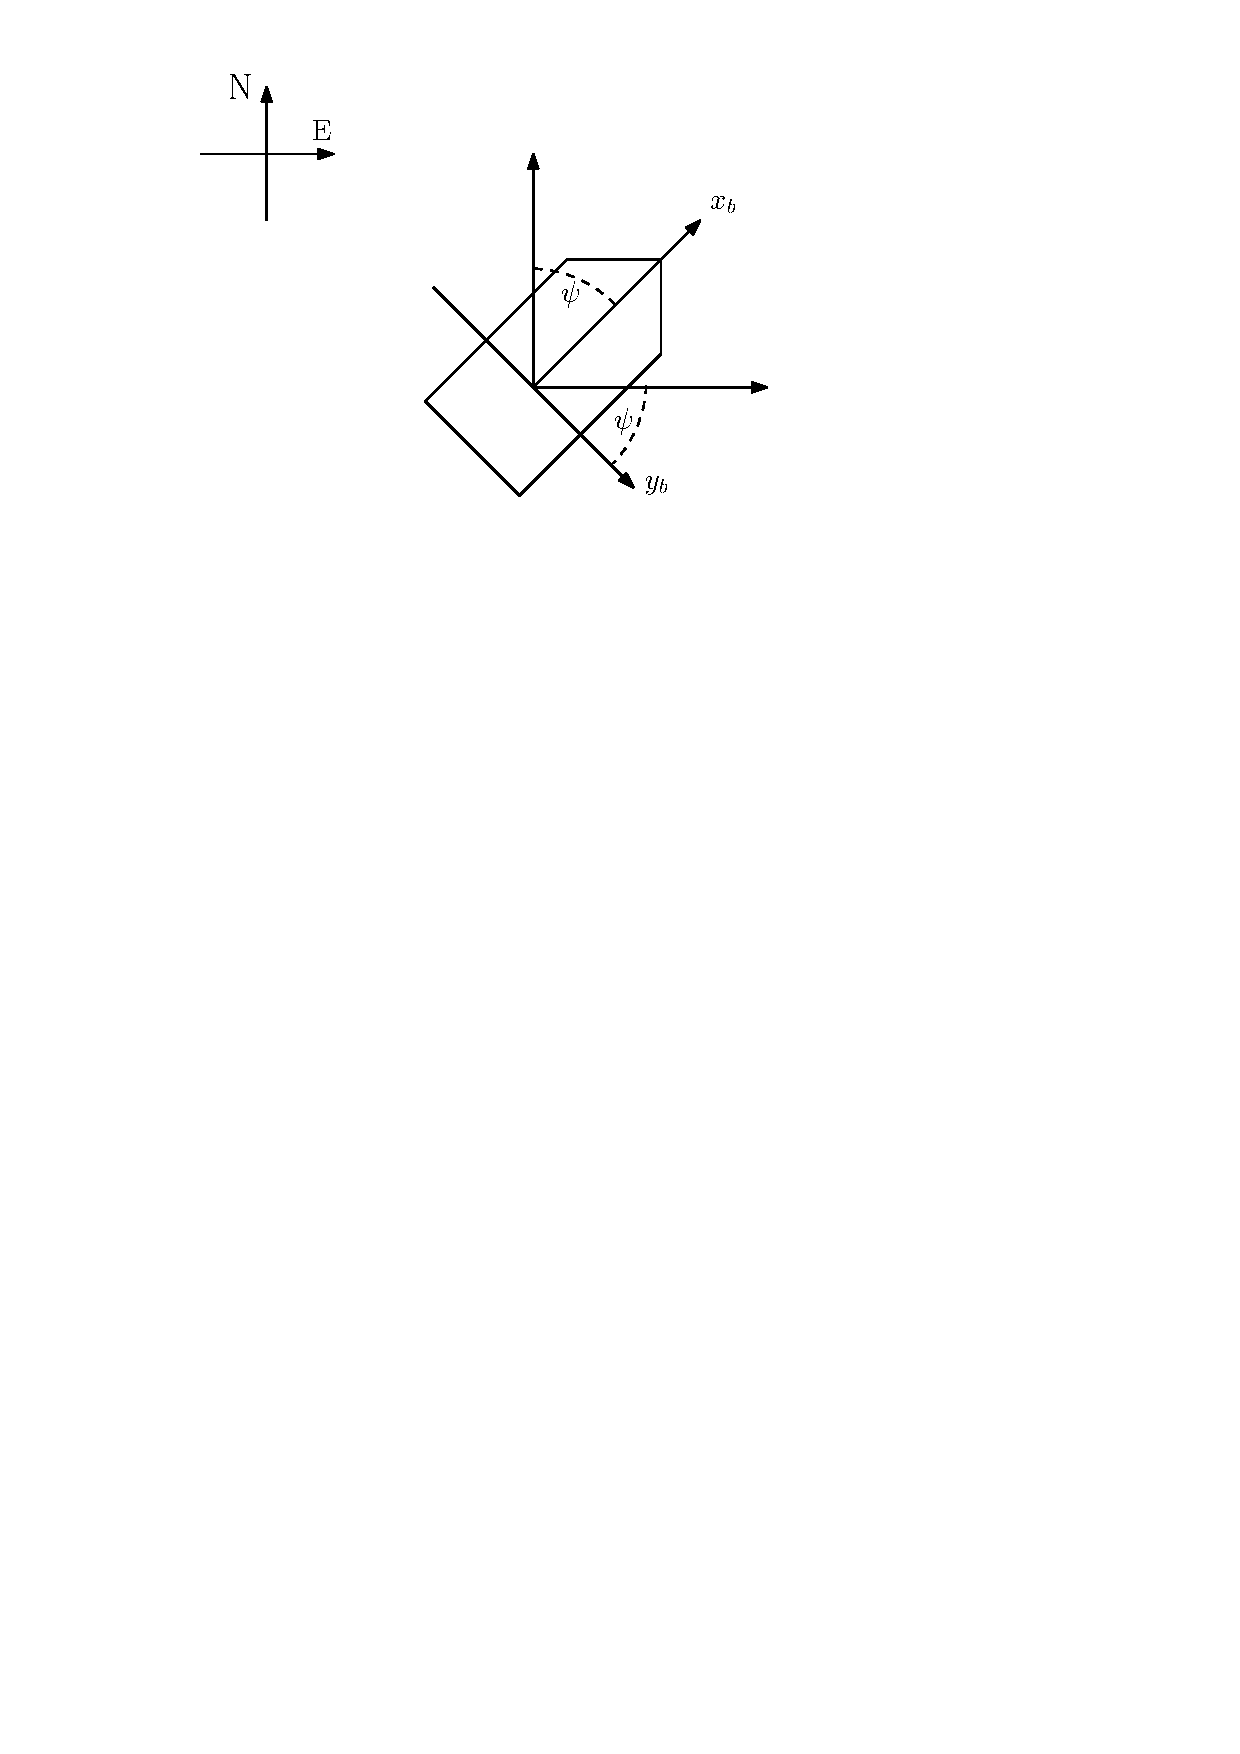
\includegraphics[width=0.5\linewidth]{Figures/boat_figure.pdf}
    \caption{BODY and NED reference frames}
    \label{fig:boat_coordsys}
\end{figure}
A dynamical model of the ship is represented by \cref{eq:dynamic_etadot} and \cref{eq:dynamic_body_vel} where the speed is low, such that some nonlinear terms as negligible
\begin{subequations}
    \begin{equation} \label{eq:dynamic_etadot}
        \dot{\boldsymbol{\eta}} = \boldsymbol{R}(\psi)\boldsymbol{\nu}
    \end{equation} 
    \begin{equation} \label{eq:dynamic_body_vel}
        \boldsymbol{M\dot{\nu} + C\nu + D\nu = \theta} + \textbf{w}
    \end{equation}
\end{subequations}
where
\begin{itemize}
    \item \textbf{M} - is the systems inertia matrix.
    \item \textbf{C} - is the Coriolis-centripetal matrix.
    \item $\boldsymbol{\tau}$ - is the vector of control inputs.
    \item \textbf{w} - is the vector of environmental disturbances.
    \item $\boldsymbol{\eta}$ - is the vector of NED positions $[x \ y \ \psi]$, where $x$ is the position in the north direction, $y$ is the position in the east-direction, and $\psi$  is the angle between the north direction and the $x_b$ axis. $\psi$ is positive clockwise.
    \item $\boldsymbol{\nu}$ - is the vector of BODY velocities $[u \ v \ r]$. Where $u$ is the velocity in the x-direction, $v$ the velocity in the y-direction and $r$ is rotation velocity about the z-axis.
\end{itemize}
The disturbances we will implement in our system are waves and current. \todo{og white noise?} The waves are considered to be high-frequency disturbances, while the current is a slowly varying disturbance. The waves representation corresponds to a spectral factorization of the wave spectrum and cam be modelled as a damped harmonic oscillator
\begin{equation*}
    \begin{bmatrix}
        \dot{x}_{w1}\\
        \dot{x}_{w2}
    \end{bmatrix} \ = \ \begin{bmatrix}
        0 & 1 \\ 
        -\omega_0^2 & -2\lambda \omega_0
    \end{bmatrix} \begin{bmatrix}
        x_{w1} \\
        x_{w1}
    \end{bmatrix} \ + \ \begin{bmatrix}
        0 \\ K_w
    \end{bmatrix} w_w \\
\end{equation*}
\begin{equation*}
    y_w = \begin{bmatrix}
        0 & 1
    \end{bmatrix} \ \begin{bmatrix}
        x_{w1} \\
        x_{w1}
    \end{bmatrix}
\end{equation*}
For the current, we will assume the only effect acting on it is the rudder angle bias. Which is modelled as in \cref{eq:b_def} where $w_b$ is the Gaussian white noise. Here it is important to note that the ship can only deviate from the reference heading with a limited number of degrees.
\newline 
\newline
Making the system into a state-space form we get
\begin{subequations} \label{eq:state_space}
    \begin{equation}
        \dot{\textbf{x}} = \textbf{Ax + B}u + \textbf{Ew}
    \end{equation}
    \begin{equation}
        y = \textbf{Cx} + v
    \end{equation}
\end{subequations}
with $\textbf{x} = [\xi_w \ \psi_w \ \psi \ r \ b]^T$, $u = \delta$ and $\textbf{w} = [w_w \ w_b]^T$. $\psi$ is the average heading, i.e. without wave disturbance. $\psi_w$ is a high-frequency component due to the wave disturbance, $\dot{\xi_w} = \psi_w$, r is the rotation velocity about the z-axis in the BODY coordinate system, and $b$ is the bias to the rudder angle. T is the systems time constant and K is the gain constant. The model used can be stated as 
\begin{subequations}
\begin{align}
        \dot{\xi_w} &= \psi_w \label{eq:xidot_def} \\
        \dot{\psi_w} &= -\omega_0^2 \xi_w - 2\lambda \omega_w \psi_w + K_w w_w \label{eq:psidot_m} \\
        \dot{\psi} &= r \label{eq:psidot} \\
        \dot{r} &= -\frac{1}{T}r + \frac{K}{T}(\delta - b) \label{eq:rdot_def} \\
        \dot{b} &= w_b \label{eq:b_def} \\
        y &= \psi + \psi_w + v \label{eq:y_def}
\end{align}
\end{subequations}
